\section{Ejercicio 8}

\subsection{Diseño}

\subsubsection{Generador de Rampa}

Primeramente, se necesitó medir de cierta manera la variación en la tensión provista por el joystick, la cual es proporcional a su posición respecto del eje. Esto se debe a que internamente el joystick cuenta con un ponteciómetro que provee entre $0\,V$ y $5\,V$. Por ende, se diseñó una rampa utilizando un circuito integrado $NE555$, la misma se utilizará para comparar tensiones. \par


La rampa representará la carga del capacitor $C_1$, dicha carga será constante debido a que el componente anteriormente mencionado está conectado con el colector del transistor PNP que está actuando como fuente de corriente. La tasa de refresco estará dada por la frecuencia de la rampa, debido a que la cátedra solicitó una tasa de entre 1 y 20 segundos, fue necesario añadir componentes variables al circuito. Para lograr dicha variación, se cambiará la pendiente de la misma, dada por $S=\frac{I_C}{C}=\frac{\Delta\,V}{\Delta\t}$. Para comenzar, se decidió fijar el valor de $C_1$ en $220\,pf$ tal que sólo sea variable $I_C$. Por otro lado, la corriente en el colector está dada por:

\begin{equation}
\frac{V_{CC}-V_E}{R_E}
\end{equation}

La tensión en el emisor está determinada por un divisor resistivo dado por:

\begin{equation}
V_E=\frac{R_4}{R_4+R_3} * V_{CC} + V_{BE}
\end{equation}

Se fijaron los valores de $R_4$ y $R_3$ en $20K\,\Omega$ y $10K\,\Omega$ respectivamente, tal que la única incógnita sea $R_E$. \par
Para obtener una tasa de refresco de entre 1 y 20 segundos





Como primer problema a solucionar, surgió que la
\begin{figure}[H]
\centering
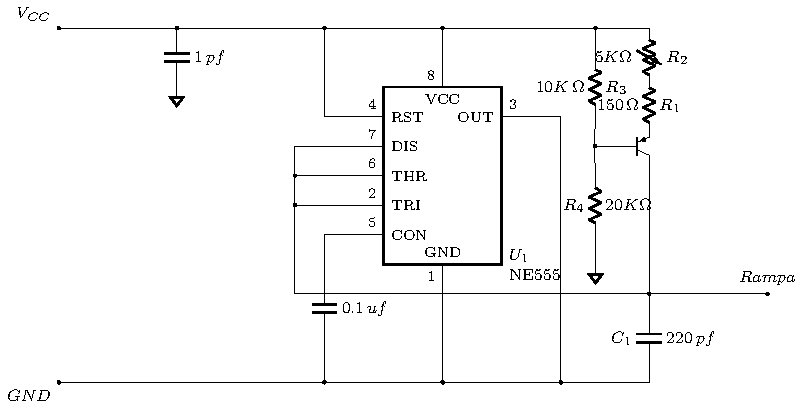
\includegraphics[scale=0.8]{Ejercicio8/Circuitos/Generador_de_rampa.pdf}
\caption{Generador de Rampa con desfasaje}
\label{fig:Generador_de_rampa}
\end{figure}

\begin{figure}[H]
\centering
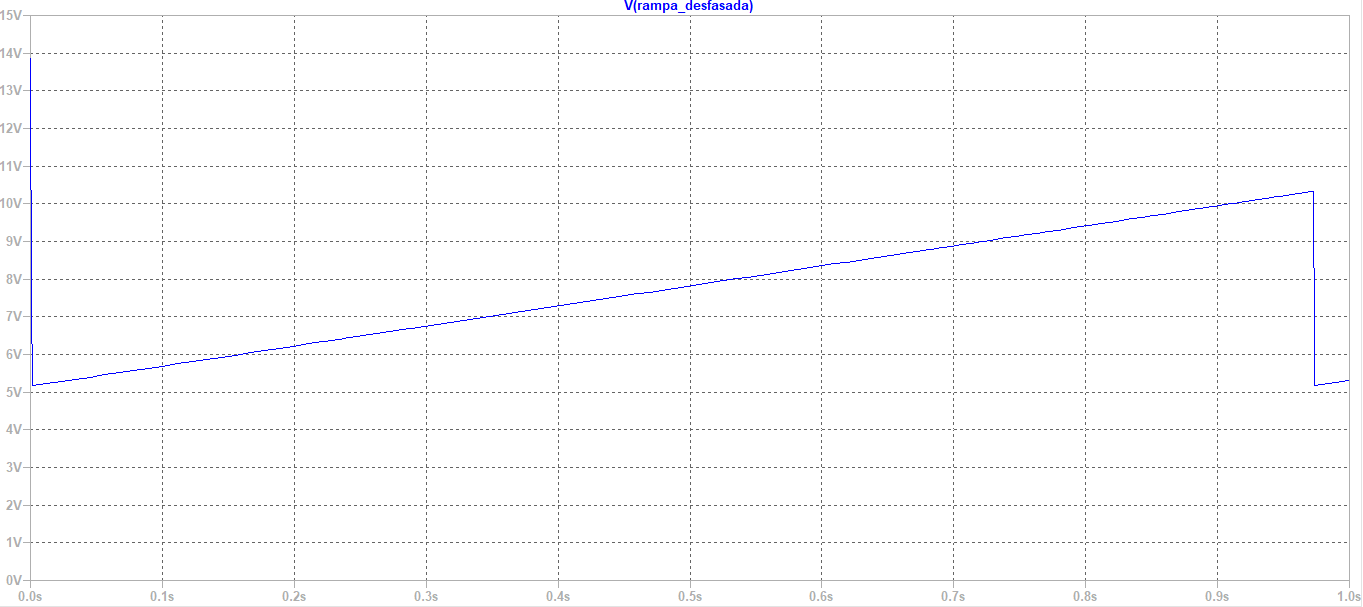
\includegraphics[width=0.7\textwidth]{Ejercicio8/Imagenes/Rampa_desfasada}
\caption{Tensión de la rampa}
\label{fig:Generador_de_rampa_LTSpice}
\end{figure}


\subsubsection{Comparador}

\begin{figure}[H]
\centering
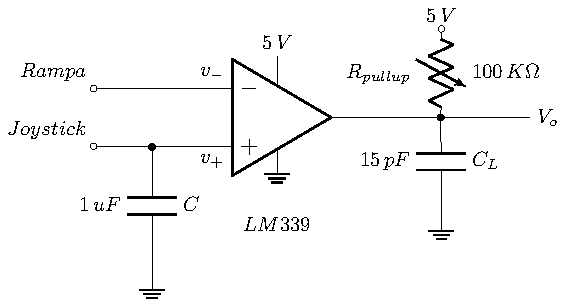
\includegraphics[scale=0.8]{Ejercicio8/Circuitos/Comparador.pdf}
\caption{Comparador}
\label{fig:Comparador}
\end{figure}

\subsubsection{Contador}

\begin{figure}[H]
\centering
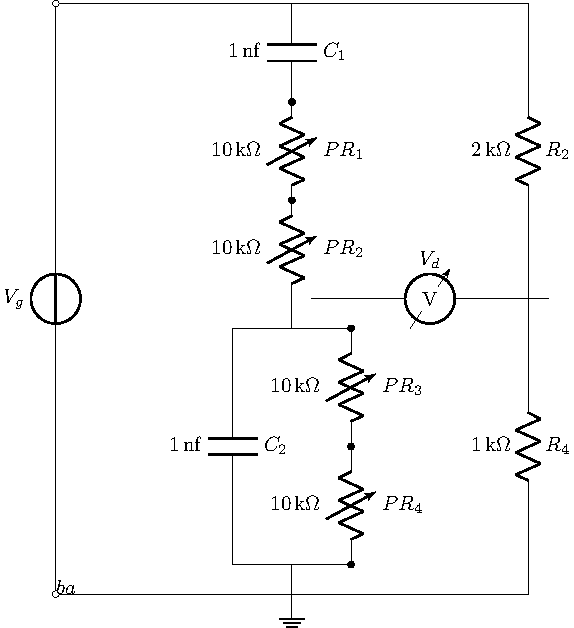
\includegraphics[scale=0.8]{Ejercicio8/Circuitos/Contador&Display.pdf}
\caption{Contador}
\label{fig:Contador&Display}
\end{figure}

\subsubsection{Clock}



\subsection{Conclusiones}